\documentclass{standalone}
\usepackage{tikz}
\usetikzlibrary{patterns}
\usetikzlibrary{positioning}
\usetikzlibrary{patterns, positioning}
\usetikzlibrary{shapes.misc}
\usepackage[outline]{contour}
\contourlength{1.5pt} 


\begin{document}
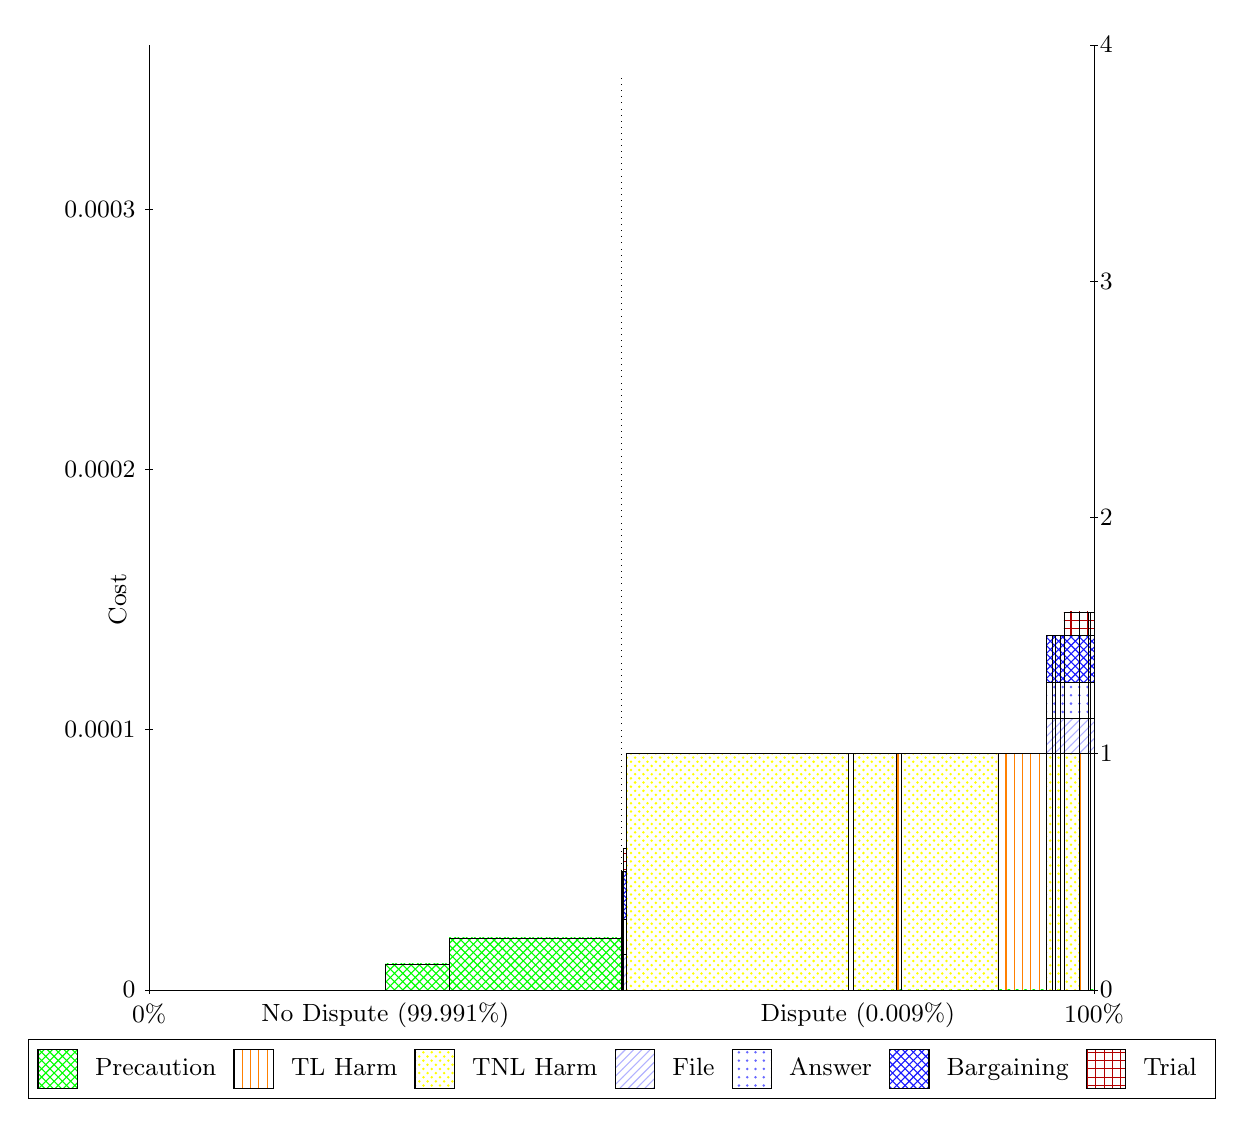
\begin{tikzpicture}
\draw[pattern=crosshatch, pattern color=green,draw=black,very thin] (4.5,2.5) rectangle (5.3092,2.8303);
\draw[pattern=crosshatch, pattern color=green,draw=black,very thin] (5.3092,2.5) rectangle (7.5,3.1607);
\draw[pattern=north east lines, pattern color=blue!30,draw=black,very thin] (7.5,2.5) rectangle (7.511,2.95);
\draw[pattern=dots,  pattern color=blue!60,draw=black,very thin] (7.5,2.95) rectangle (7.511,3.4);
\draw[pattern=crosshatch,      pattern color=blue!90,draw=black,very thin] (7.5,3.4) rectangle (7.511,4);
\draw[pattern=crosshatch, pattern color=green,draw=black,very thin] (7.511,2.5) rectangle (7.5235,2.5);
\draw[pattern=north east lines, pattern color=blue!30,draw=black,very thin] (7.511,2.5) rectangle (7.5235,2.95);
\draw[pattern=dots,  pattern color=blue!60,draw=black,very thin] (7.511,2.95) rectangle (7.5235,3.4);
\draw[pattern=crosshatch,      pattern color=blue!90,draw=black,very thin] (7.511,3.4) rectangle (7.5235,4);
\draw[pattern=north east lines, pattern color=blue!30,draw=black,very thin] (7.5235,2.5) rectangle (7.5545,2.95);
\draw[pattern=dots,  pattern color=blue!60,draw=black,very thin] (7.5235,2.95) rectangle (7.5545,3.4);
\draw[pattern=crosshatch,      pattern color=blue!90,draw=black,very thin] (7.5235,3.4) rectangle (7.5545,4);
\draw[pattern=grid,            pattern color=red!70!black,draw=black,very thin] (7.5235,4) rectangle (7.5545,4.3);
\draw[pattern=crosshatch, pattern color=green,draw=black,very thin] (7.5545,2.5) rectangle (7.563,2.5);
\draw[pattern=north east lines, pattern color=blue!30,draw=black,very thin] (7.5545,2.5) rectangle (7.563,2.95);
\draw[pattern=dots,  pattern color=blue!60,draw=black,very thin] (7.5545,2.95) rectangle (7.563,3.4);
\draw[pattern=crosshatch,      pattern color=blue!90,draw=black,very thin] (7.5545,3.4) rectangle (7.563,4);
\draw[pattern=grid,            pattern color=red!70!black,draw=black,very thin] (7.5545,4) rectangle (7.563,4.3);
\draw[pattern=crosshatch dots, pattern color=yellow,draw=black,very thin] (7.563,2.5) rectangle (10.378,5.5);
\draw[pattern=vertical lines, pattern color=orange,draw=black,very thin] (10.378,2.5) rectangle (10.447,5.5);
\draw[pattern=crosshatch, pattern color=green,draw=black,very thin] (10.447,2.5) rectangle (10.993,2.5);
\draw[pattern=crosshatch dots, pattern color=yellow,draw=black,very thin] (10.447,2.5) rectangle (10.993,5.5);
\draw[pattern=crosshatch, pattern color=green,draw=black,very thin] (10.993,2.5) rectangle (11.057,2.5);
\draw[pattern=vertical lines, pattern color=orange,draw=black,very thin] (10.993,2.5) rectangle (11.057,5.5);
\draw[pattern=crosshatch, pattern color=green,draw=black,very thin] (11.057,2.5) rectangle (12.278,2.5001);
\draw[pattern=crosshatch dots, pattern color=yellow,draw=black,very thin] (11.057,2.5001) rectangle (12.278,5.5001);
\draw[pattern=crosshatch, pattern color=green,draw=black,very thin] (12.278,2.5) rectangle (12.896,2.5001);
\draw[pattern=vertical lines, pattern color=orange,draw=black,very thin] (12.278,2.5001) rectangle (12.896,5.5001);
\draw[pattern=crosshatch dots, pattern color=yellow,draw=black,very thin] (12.896,2.5) rectangle (12.965,5.5);
\draw[pattern=north east lines, pattern color=blue!30,draw=black,very thin] (12.896,5.5) rectangle (12.965,5.95);
\draw[pattern=dots,  pattern color=blue!60,draw=black,very thin] (12.896,5.95) rectangle (12.965,6.4);
\draw[pattern=crosshatch,      pattern color=blue!90,draw=black,very thin] (12.896,6.4) rectangle (12.965,7);
\draw[pattern=vertical lines, pattern color=orange,draw=black,very thin] (12.965,2.5) rectangle (13.006,5.5);
\draw[pattern=north east lines, pattern color=blue!30,draw=black,very thin] (12.965,5.5) rectangle (13.006,5.95);
\draw[pattern=dots,  pattern color=blue!60,draw=black,very thin] (12.965,5.95) rectangle (13.006,6.4);
\draw[pattern=crosshatch,      pattern color=blue!90,draw=black,very thin] (12.965,6.4) rectangle (13.006,7);
\draw[pattern=crosshatch, pattern color=green,draw=black,very thin] (13.006,2.5) rectangle (13.065,2.5);
\draw[pattern=crosshatch dots, pattern color=yellow,draw=black,very thin] (13.006,2.5) rectangle (13.065,5.5);
\draw[pattern=north east lines, pattern color=blue!30,draw=black,very thin] (13.006,5.5) rectangle (13.065,5.95);
\draw[pattern=dots,  pattern color=blue!60,draw=black,very thin] (13.006,5.95) rectangle (13.065,6.4);
\draw[pattern=crosshatch,      pattern color=blue!90,draw=black,very thin] (13.006,6.4) rectangle (13.065,7);
\draw[pattern=crosshatch, pattern color=green,draw=black,very thin] (13.065,2.5) rectangle (13.116,2.5);
\draw[pattern=vertical lines, pattern color=orange,draw=black,very thin] (13.065,2.5) rectangle (13.116,5.5);
\draw[pattern=north east lines, pattern color=blue!30,draw=black,very thin] (13.065,5.5) rectangle (13.116,5.95);
\draw[pattern=dots,  pattern color=blue!60,draw=black,very thin] (13.065,5.95) rectangle (13.116,6.4);
\draw[pattern=crosshatch,      pattern color=blue!90,draw=black,very thin] (13.065,6.4) rectangle (13.116,7);
\draw[pattern=crosshatch dots, pattern color=yellow,draw=black,very thin] (13.116,2.5) rectangle (13.308,5.5);
\draw[pattern=north east lines, pattern color=blue!30,draw=black,very thin] (13.116,5.5) rectangle (13.308,5.95);
\draw[pattern=dots,  pattern color=blue!60,draw=black,very thin] (13.116,5.95) rectangle (13.308,6.4);
\draw[pattern=crosshatch,      pattern color=blue!90,draw=black,very thin] (13.116,6.4) rectangle (13.308,7);
\draw[pattern=grid,            pattern color=red!70!black,draw=black,very thin] (13.116,7) rectangle (13.308,7.3);
\draw[pattern=vertical lines, pattern color=orange,draw=black,very thin] (13.308,2.5) rectangle (13.426,5.5);
\draw[pattern=north east lines, pattern color=blue!30,draw=black,very thin] (13.308,5.5) rectangle (13.426,5.95);
\draw[pattern=dots,  pattern color=blue!60,draw=black,very thin] (13.308,5.95) rectangle (13.426,6.4);
\draw[pattern=crosshatch,      pattern color=blue!90,draw=black,very thin] (13.308,6.4) rectangle (13.426,7);
\draw[pattern=grid,            pattern color=red!70!black,draw=black,very thin] (13.308,7) rectangle (13.426,7.3);
\draw[pattern=crosshatch, pattern color=green,draw=black,very thin] (13.426,2.5) rectangle (13.452,2.5);
\draw[pattern=crosshatch dots, pattern color=yellow,draw=black,very thin] (13.426,2.5) rectangle (13.452,5.5);
\draw[pattern=north east lines, pattern color=blue!30,draw=black,very thin] (13.426,5.5) rectangle (13.452,5.95);
\draw[pattern=dots,  pattern color=blue!60,draw=black,very thin] (13.426,5.95) rectangle (13.452,6.4);
\draw[pattern=crosshatch,      pattern color=blue!90,draw=black,very thin] (13.426,6.4) rectangle (13.452,7);
\draw[pattern=grid,            pattern color=red!70!black,draw=black,very thin] (13.426,7) rectangle (13.452,7.3);
\draw[pattern=crosshatch, pattern color=green,draw=black,very thin] (13.452,2.5) rectangle (13.5,2.5);
\draw[pattern=vertical lines, pattern color=orange,draw=black,very thin] (13.452,2.5) rectangle (13.5,5.5);
\draw[pattern=north east lines, pattern color=blue!30,draw=black,very thin] (13.452,5.5) rectangle (13.5,5.95);
\draw[pattern=dots,  pattern color=blue!60,draw=black,very thin] (13.452,5.95) rectangle (13.5,6.4);
\draw[pattern=crosshatch,      pattern color=blue!90,draw=black,very thin] (13.452,6.4) rectangle (13.5,7);
\draw[pattern=grid,            pattern color=red!70!black,draw=black,very thin] (13.452,7) rectangle (13.5,7.3);
\draw[black,very thin] (1.5,2.5) -- (1.5,14.5);
\node[font=\small,rotate=90,text=black, anchor=center] at (1.1, 7.4549) {Cost};
\draw[black,very thin] (1.45,2.5) -- (1.55,2.5);
\node[font=\small,text=black, anchor=east] at (1.45, 2.5) {0};
\draw[black,very thin] (1.45,5.8033) -- (1.55,5.8033);
\node[font=\small,text=black, anchor=east] at (1.45, 5.8033) {0.0001};
\draw[black,very thin] (1.45,9.1066) -- (1.55,9.1066);
\node[font=\small,text=black, anchor=east] at (1.45, 9.1066) {0.0002};
\draw[black,very thin] (1.45,12.41) -- (1.55,12.41);
\node[font=\small,text=black, anchor=east] at (1.45, 12.41) {0.0003};

\draw[black,dotted,very thin] (7.5,2.86) -- (7.5,14.14);
\draw[black,very thin] (13.5,2.5) -- (13.5,14.5);
\draw[black,very thin] (13.45,2.5) -- (13.55,2.5);
\node[font=\small,text=black, anchor=west] at (13.45, 2.5) {0};
\draw[black,very thin] (13.45,5.5) -- (13.55,5.5);
\node[font=\small,text=black, anchor=west] at (13.45, 5.5) {1};
\draw[black,very thin] (13.45,8.5) -- (13.55,8.5);
\node[font=\small,text=black, anchor=west] at (13.45, 8.5) {2};
\draw[black,very thin] (13.45,11.5) -- (13.55,11.5);
\node[font=\small,text=black, anchor=west] at (13.45, 11.5) {3};
\draw[black,very thin] (13.45,14.5) -- (13.55,14.5);
\node[font=\small,text=black, anchor=west] at (13.45, 14.5) {4};

\draw[black,very thin] (1.5,2.5) -- (13.5,2.5);
\draw[black,very thin] (1.5,2.45) -- (1.5,2.55);
\node[font=\small,text=black, anchor=north] at (1.5, 2.45) {0\%};
\draw[black,very thin] (13.5,2.45) -- (13.5,2.55);
\node[font=\small,text=black, anchor=north] at (13.5, 2.45) {100\%};

\node[font=\small,text=black,anchor=south] at (4.5, 1.9) {No\ Dispute\ (99.991\%)};
\node[font=\small,text=black,anchor=south] at (10.5, 1.9) {Dispute\ (0.009\%)};
\draw (7.5,2.5) node (B) {};
\begin{scope}[align=center]
\matrix[scale=0.5,draw=black,below=0.5cm of B,nodes={draw},column sep=0.1cm]{
\node[rectangle,draw,minimum width=0.5cm,minimum height=0.5cm,pattern=crosshatch, pattern color=green]{}; & \node[draw=none,font=\small,text=black]{Precaution}; &
\node[rectangle,draw,minimum width=0.5cm,minimum height=0.5cm,pattern=vertical lines, pattern color=orange]{}; & \node[draw=none,font=\small,text=black]{TL Harm}; &
\node[rectangle,draw,minimum width=0.5cm,minimum height=0.5cm,pattern=crosshatch dots, pattern color=yellow]{}; & \node[draw=none,font=\small,text=black]{TNL Harm}; &
\node[rectangle,draw,minimum width=0.5cm,minimum height=0.5cm,pattern=north east lines, pattern color=blue!30]{}; & \node[draw=none,font=\small,text=black]{File}; &
\node[rectangle,draw,minimum width=0.5cm,minimum height=0.5cm,pattern=dots,  pattern color=blue!60]{}; & \node[draw=none,font=\small,text=black]{Answer}; &
\node[rectangle,draw,minimum width=0.5cm,minimum height=0.5cm,pattern=crosshatch,      pattern color=blue!90]{}; & \node[draw=none,font=\small,text=black]{Bargaining}; &
\node[rectangle,draw,minimum width=0.5cm,minimum height=0.5cm,pattern=grid,            pattern color=red!70!black]{}; & \node[draw=none,font=\small,text=black]{Trial}; \\\\
};\end{scope}

\end{tikzpicture}
\end{document}